\documentclass[conference]{IEEEtran}

\usepackage{amsmath}
\usepackage{array}
\usepackage{booktabs}
\usepackage{cite}
\usepackage{graphicx}
\usepackage{url}

\begin{document}

\title{Hardware/Software Co-Design for FPGA-Accelerated MAYO Signature Verification}

\author{
\IEEEauthorblockN{Kowsyap Pranay Kumar Musumuri}
\IEEEauthorblockA{G01503265\\
ECE 615, George Mason University}
}

\maketitle
\thispagestyle{plain}
\pagestyle{plain}

\begin{abstract}
This report presents a hardware/software co-design implementation for verifying MAYO post-quantum digital signatures on a Zybo Z7-10 Zynq-7000 FPGA platform. The design targets the MAYO Security Level 1 Set 2 parameter instances for both Round 1 and Round 2. The ARM Cortex-A9 processing system performs compact public-key expansion using AES-128-CTR and derives the verification target with SHAKE256, while the programmable logic accelerates the dominant multivariate quadratic evaluation over \(F_q\), with \(q=16\). The accelerator receives the decoded signature and expanded public key through AXI DMA, computes the verification vector, and returns the result to software for comparison against the target vector. Known Answer Tests pass for both supported parameter sets, and on-board profiling shows that the programmable-logic computation takes approximately 1.2 microseconds. The current end-to-end latency is dominated by transferring the expanded public key, which is roughly 99--106 kB depending on the MAYO round.
\end{abstract}

\begin{IEEEkeywords}
post-quantum cryptography, MAYO, FPGA, Zynq, hardware/software co-design, \(F_q\), digital signatures
\end{IEEEkeywords}

\section{Introduction}
Post-quantum cryptography addresses the risk that large-scale quantum computers could break classical public-key cryptosystems based on integer factorization and discrete logarithms. MAYO is a multivariate quadratic signature scheme whose verification procedure is built around finite-field arithmetic over \(F_q\), where \(q=16\). This arithmetic maps well to FPGA fabric because the computation is structured, bit-level, and highly parallel.

The project implements a MAYO verification accelerator on the Zybo Z7-10 board. The design splits the verification workload across the Zynq processing system (PS) and programmable logic (PL). Software performs the cryptographic expansion and hashing steps that are already available as compact C implementations, while hardware performs the repeated quadratic matrix-vector evaluation that dominates the arithmetic portion of verification.

\section{MAYO Verification Background}
MAYO is a post-quantum digital signature candidate submitted to the NIST additional signature process \cite{mayo,nistpqc}. It is specified as a multivariate quadratic signature scheme over \(F_q\), where \(q=16\). The public map is a sequence of \(m\) homogeneous quadratic polynomials,
\begin{equation}
P(x)=(p_1(x),\ldots,p_m(x)):F_q^n\rightarrow F_q^m,
\end{equation}
and verification recomputes this public map on the signature-derived vector and checks it against a message-derived digest target. The Round 1 and Round 2 specifications describe the same verification structure, with different parameter sets and encoding details \cite{mayo-r1,mayo-r2}.

At a high level, verification proceeds as follows:
\begin{enumerate}
\item Expand the compact public key (CPK) into the expanded public key (EPK).
\item Derive target vector \(T\) from the message and salt using SHAKE256.
\item Decode the signature into \(k\) vectors over \(F_q\).
\item Evaluate the MAYO public map \(Y=P(s)\) over \(F_q\).
\item Accept the signature if \(Y=T\).
\end{enumerate}

The expanded public key contains \(m\) block-structured matrices. For equation \(a\), the matrix used by verification is
\begin{equation}
P_a =
\begin{bmatrix}
P^{(1)}_a & P^{(2)}_a \\
0 & P^{(3)}_a
\end{bmatrix},
\end{equation}
where \(P^{(1)}_a\in F_q^{(n-o)\times(n-o)}\) and \(P^{(3)}_a\in F_q^{o\times o}\) are upper-triangular blocks, and \(P^{(2)}_a\in F_q^{(n-o)\times o}\) is rectangular. The compact public key stores a seed and \(P^{(3)}\); \(P^{(1)}\) and \(P^{(2)}\) are generated from the seed with AES-128-CTR during public-key expansion. This layout reduces key storage and guides how the hardware decoder stores the expanded key.

The MAYO verifier first splits the decoded signature into \(k\) vectors \(s_0,\ldots,s_{k-1}\), each in \(F_q^n\). It then loops over the triangular set of vector pairs \((i,j)\), so there are \(k(k+1)/2\) pair contributions. For each pair, the verifier forms a vector \(u_{i,j}\in F_q^m\) whose \(a\)-th element is
\begin{equation}
u_{i,j,a} =
\begin{cases}
s_i^T P_a s_i, & i=j,\\
s_i^T P_a s_j + s_j^T P_a s_i, & i\ne j.
\end{cases}
\end{equation}
The final result is accumulated as
\begin{equation}
Y=\sum_{\ell=0}^{k(k+1)/2-1} E^\ell u_\ell,
\end{equation}
where \(E\) represents multiplication by \(z\) in \(F_q[z]/f(z)\). The specifications note that these \(E^\ell\) products can be handled efficiently by accumulating in polynomial form and reducing once modulo \(f(z)\), which is the idea reflected in the hardware reduction stage.

For this implementation, the main Round 1 and Round 2 differences are not the high-level verifier loop but the parameters and encodings around it. Both rounds still expand \(P^{(1)}\) and \(P^{(2)}\) from a public seed, decode \(P^{(3)}\), derive \(T\), and evaluate the same triangular \(k=4\) pair schedule. Round 1 Set 2 uses \(n=78,o=18,d=60\), a 98,592-byte EPK, and the specification's bit-sliced matrix encoding, so the hardware includes a bit-sliced conversion path for loaded public-key vectors. Round 2 Set 2 changes to \(n=81,o=17,d=64\), increases the EPK to 106,272 bytes, and uses the newer interleaved matrix encoding that the hardware can pass through more directly. The larger vinegar dimension in Round 2 increases the P1 region and slightly raises LUT utilization, while the same \(m=64\), \(k=4\), salt length, and digest length keep the target vector width and accumulator output interface unchanged.

Fig.~\ref{fig:algorithm} summarizes the verification flow used to partition work between software and hardware.

\begin{figure}[t]
\centering
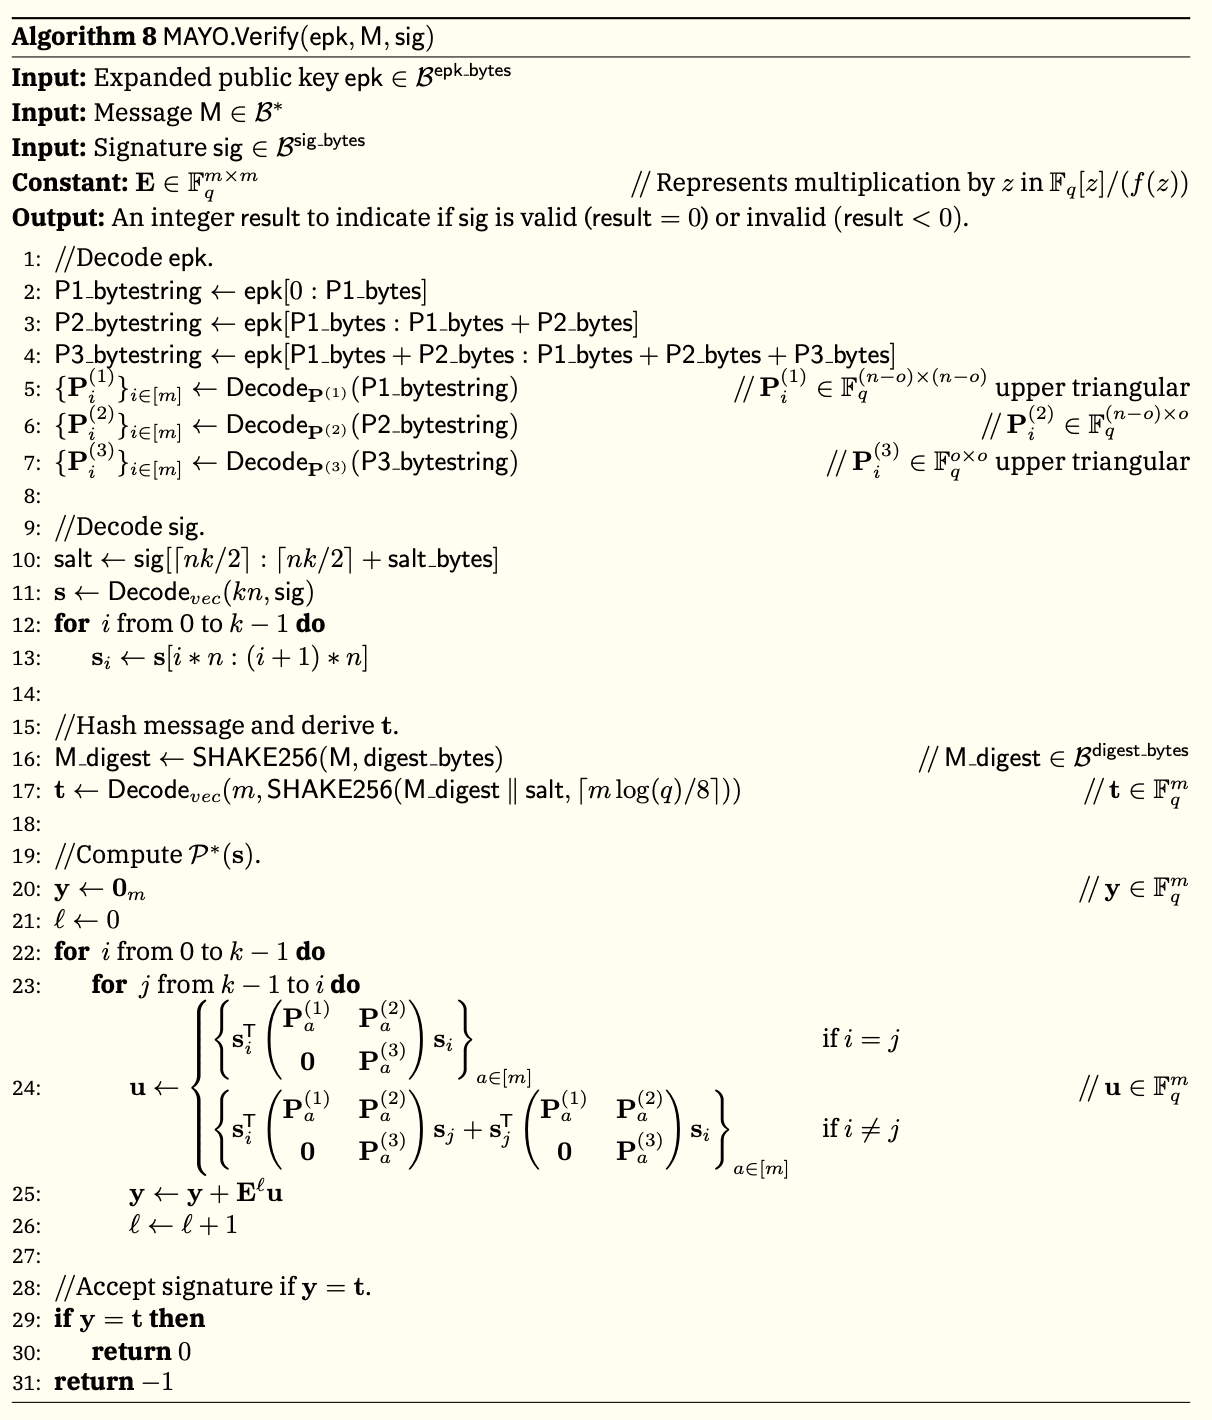
\includegraphics[width=\linewidth]{figures/algorithm.png}
\caption{MAYO verification algorithm used as the basis for the accelerator design.}
\label{fig:algorithm}
\end{figure}

\section{Supported Parameters}
The implementation supports MAYO Security Level 1 Set 2 for both Round 1 and Round 2. The VHDL package selects the parameter set through the top-level generic \texttt{round}, and the embedded C support code defines matching software-side constants. Table~\ref{tab:params} summarizes the supported parameter sets.

\begin{table}[t]
\centering
\caption{Supported MAYO Security Level 1 Set 2 Parameters}
\label{tab:params}
\begin{tabular}{lcc}
\toprule
Parameter & Round 1 & Round 2 \\
\midrule
\(m\) equations & 64 & 64 \\
\(n\) variables & 78 & 81 \\
\(o\) oil variables & 18 & 17 \\
\(k\) signature vectors & 4 & 4 \\
\(d=n-o\) & 60 & 64 \\
CPK bytes & 5,488 & 4,912 \\
EPK bytes & 98,592 & 106,272 \\
Signature bytes & 180 & 186 \\
Salt bytes & 24 & 24 \\
Digest bytes & 32 & 32 \\
\bottomrule
\end{tabular}
\end{table}

Round 2 has a larger vinegar dimension and a larger EPK, which increases both logic pressure and transfer volume. This difference is visible in the implementation reports: Round 2 uses more LUTs than Round 1 while BRAM usage remains the same.

\section{System Architecture}
Fig.~\ref{fig:arch} shows the top-level Zynq integration around the processing system, AXI DMA, FIFO buffering, and custom MAYO verification hardware IP. The Zynq-7000 platform combines an ARM processing system with programmable logic fabric, which matches the project split between software-side cryptographic setup and hardware-side quadratic evaluation \cite{xilinxzynq}. A host computer sends message, compact public key, and signature fields to the Zynq PS over UART. The bare-metal C application expands the public key with AES-128-CTR, derives the target \(T\) with SHAKE256, and packs the signature payload and EPK into a DMA buffer. The buffer is streamed to the PL accelerator through AXI DMA.

\begin{figure}[t]
\centering
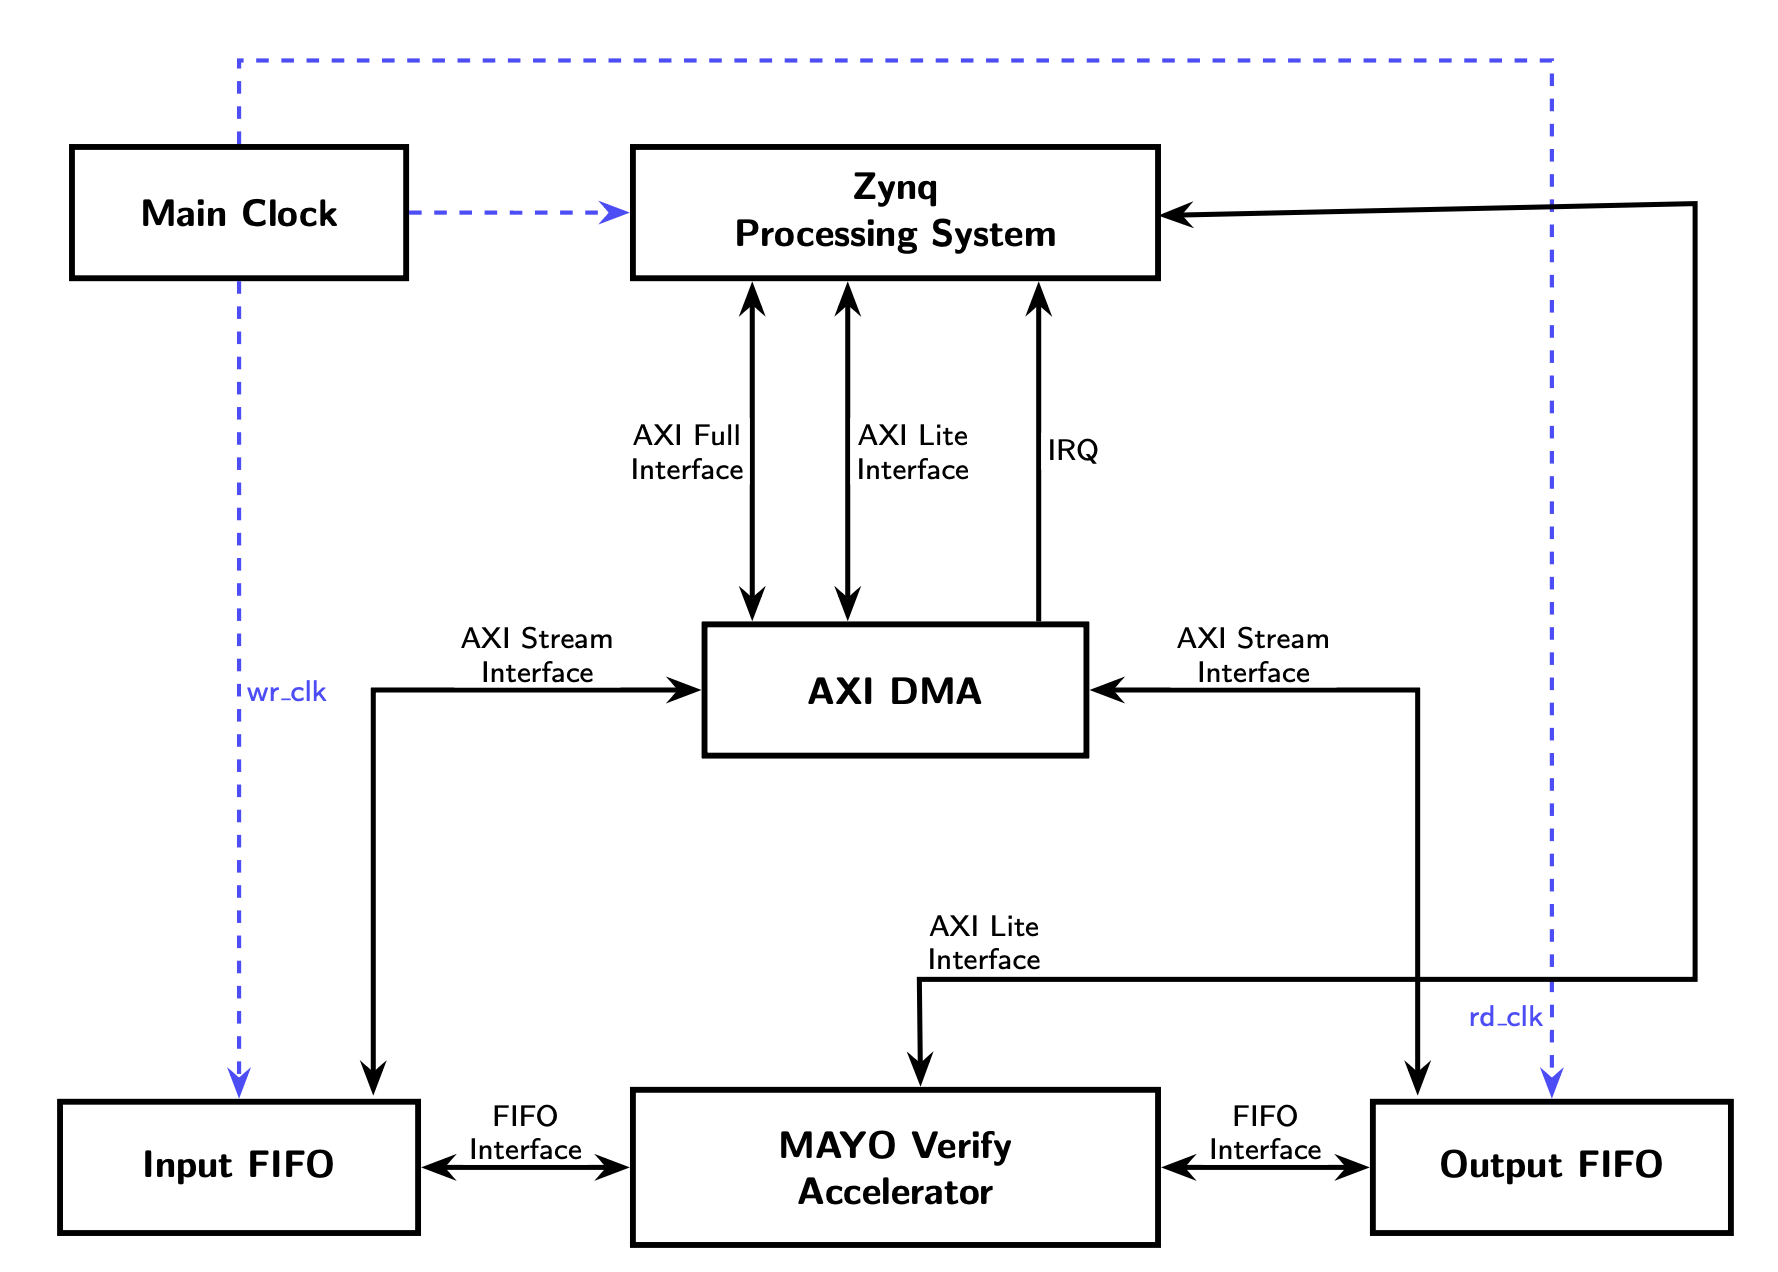
\includegraphics[width=\linewidth]{figures/arch.png}
\caption{Top-level Zynq architecture connecting the processing system, AXI DMA, FIFO buffers, and custom MAYO verification hardware IP.}
\label{fig:arch}
\end{figure}

The accelerator output is the packed \(m/2=32\)-byte vector \(Y\). Software receives this vector, corrects the byte order, and compares it with the target vector. A one-byte UART response indicates whether the signature is valid.

\section{Hardware Design}
The PL design is written in VHDL. The top-level \texttt{mayo\_verify} entity instantiates three main computational blocks: \texttt{sig\_decoder}, \texttt{epk\_decoder}, and \texttt{quad\_accumulator}. It also instantiates \texttt{data\_storage}, which holds signature vectors and key-derived intermediate values in RAM banks.

\subsection{Control FSM}
The top-level hardware controller follows the sequence shown in Fig.~\ref{fig:fsm}. After reset, the PS writes the control register to assert \texttt{calc}. The hardware then decodes the signature, decodes and stores the expanded public key, runs the quadratic accumulator, and finally asserts \texttt{done}.

\begin{figure}[t]
\centering
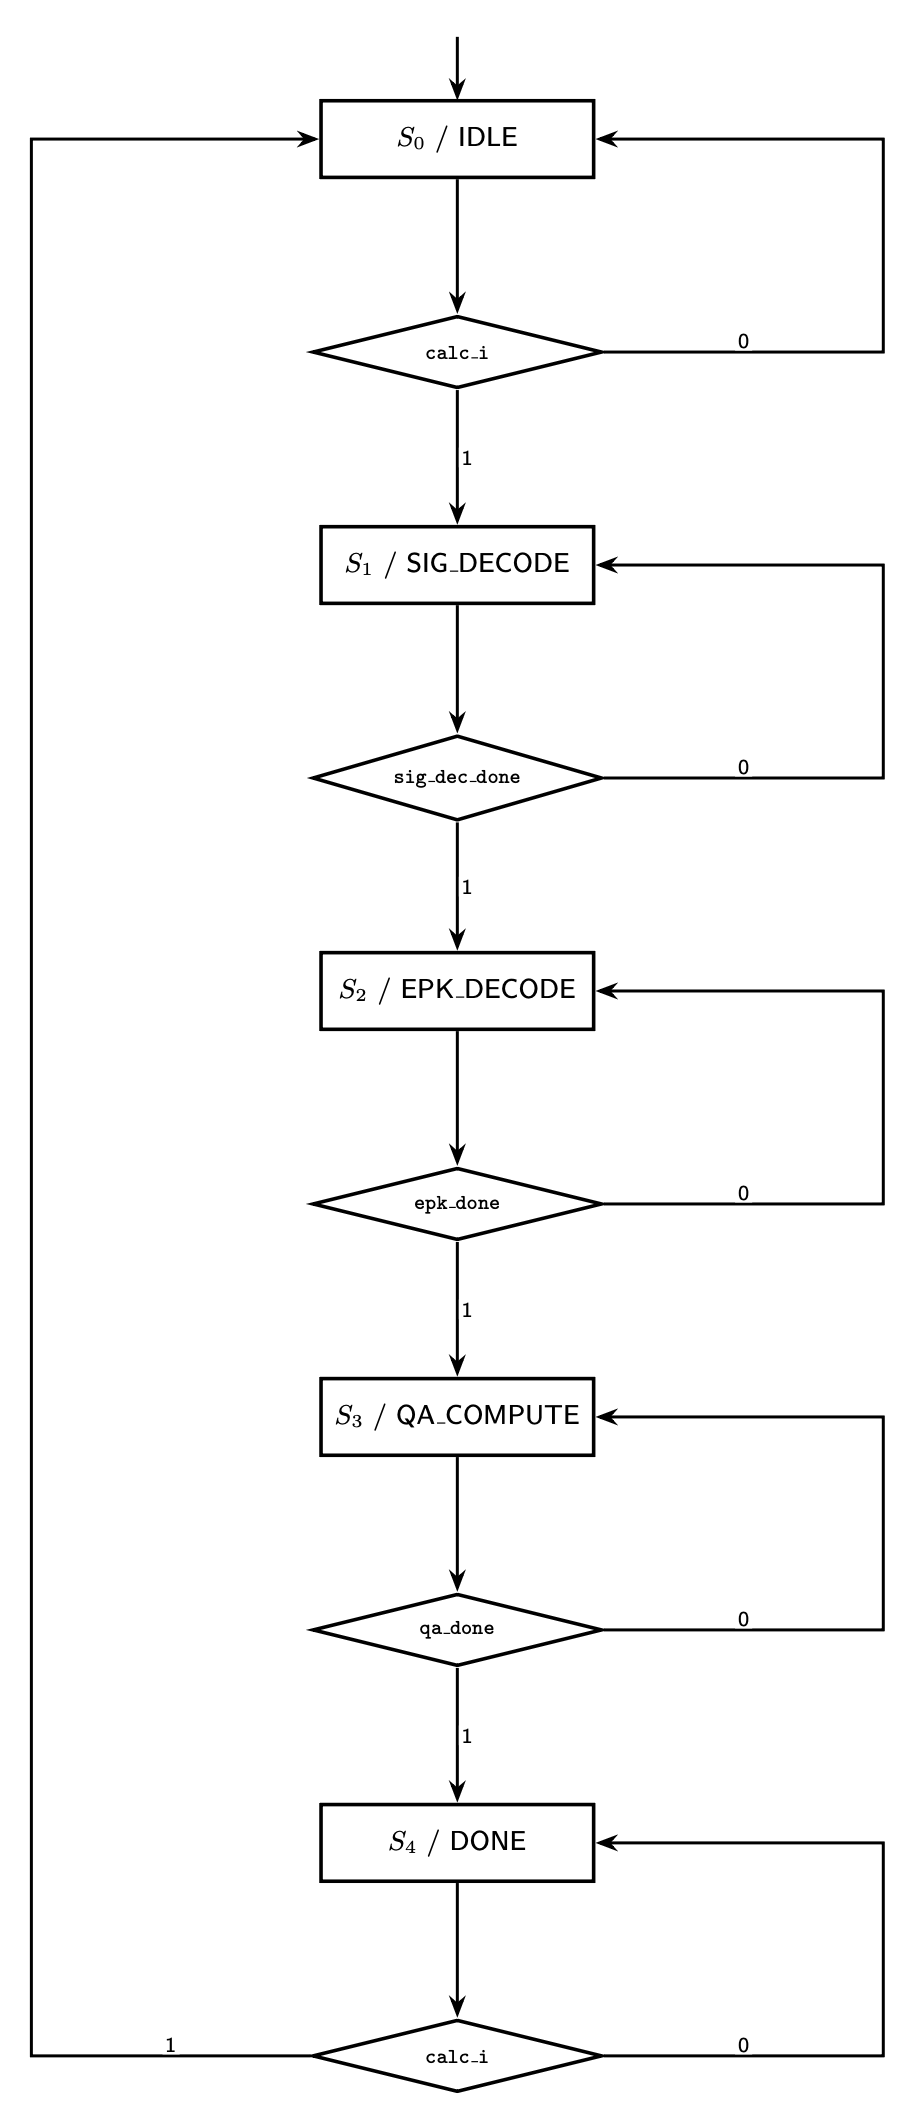
\includegraphics[width=0.66\linewidth]{figures/fsm.png}
\caption{Top-level accelerator finite-state machine.}
\label{fig:fsm}
\end{figure}

\subsection{AXI Interfaces}
The \texttt{mayo\_verify\_accelerator} wrapper exposes one AXI-Lite control/status register and AXI Stream input/output ports. Register bit 0 starts computation when written as one, and the same register reports completion when the accelerator reaches the done state. The AXI Stream slave receives the packed signature payload followed by the EPK; the AXI Stream master returns the computed \(Y\) vector.

\subsection{Signature Decoder}
The \texttt{sig\_decoder} receives the signature as 64-bit AXI Stream words and reconstructs the signature vectors used by the MAYO verifier. The incoming words are passed through serial-in parallel-out FIFO logic until enough nibbles have been collected to form one \(n\)-element vector register. That vector is stored as \(s_i\), and the same process repeats until all \(k=4\) signature vector registers \(s_i\), for \(i=0,\ldots,k-1\), are available to the later matrix-vector computation. Once the four vectors are loaded, the decoder asserts \texttt{sig\_dec\_done}.

\subsection{Expanded-Key Decoder}
The \texttt{epk\_decoder} streams the EPK and reconstructs the \(P^{(1)}\), \(P^{(2)}\), and \(P^{(3)}\) matrix regions. Its controller has separate state ranges for \(P1\), \(P2\), and \(P3\). For \(P1\) and \(P3\), the row and column counters follow the upper-triangular matrix structure by initializing \(j=i\). For \(P2\), the controller starts the column counter at \(d=n-o\), because \(P2\) spans the vinegar-to-oil block. The datapath groups four 64-bit stream words into one \(m\)-element packed vector, since \(m=64\) field values occupy 256 bits. A packed vector represents one matrix coordinate across all \(m\) public-map equations: for a fixed row and column \((i,j)\), it contains the \((i,j)\)-th coefficient from each of the \(m\) matrices. Round 1 uses the \texttt{bit\_sliced\_vector} conversion before storage, while Round 2 can forward the packed vector directly according to its encoding.

Instead of storing the EPK as \(m\) raw matrices and recomputing all products later, the hardware precomputes matrix-vector products while the key is being decoded. For each signature vector \(s_i\), \(i=0,\ldots,k-1\), the packed \(P_a\) coefficients are multiplied against the relevant nibble of \(s_i\) using parallel multiplier resources. The products are accumulated in a multiply-accumulate style to form \(P_a s_i\), and the result for each \(s_i\) is stored in its own RAM bank. These stored \(P_a s_i\) values are then reused by the later quadratic stage when computing terms of the form \(s_i^T P_a s_j\).

\subsection{Quadratic Accumulator}
The \texttt{quad\_accumulator} performs the arithmetic core of verification. The MAYO specification expresses verification as a triangular pair loop over \((i,j)\), which would require \(k(k+1)/2\) pair evaluations. In this design, the explicit \(j\) iteration is largely removed by the EPK-loading precomputation. The hardware has \(k\) RAM resources that store the \(P_a s_i\) values needed by the later dot products, so for a given outer index \(i\), the required contributions with all valid \(j\) values can be formed in parallel and combined with an XOR tree. For \(k=4\), this reduces the accumulator schedule from ten pair iterations to four outer \(i\) iterations.

For a diagonal term, the accumulator multiplies stored \(P_a s_i\) data with the matching signature vector to form \(s_i^T P_a s_i\). For off-diagonal terms, it uses the precomputed RAM contents for the other signature vectors to form the symmetric terms needed for \(s_i^T P_a s_j+s_j^T P_a s_i\). Since each stored value is packed across all \(m\) equations, the hardware works on many public-map outputs in parallel while also combining the \(j\)-dependent lanes for the current \(i\) through XOR reduction.

After the \(u\) contribution is produced for each outer \(i\), the datapath applies the same \(E^\ell\) weighting used in the MAYO verification equation by shifting the packed result. For \(k=4\), the four outer iterations are shifted by 0, 4, 7, and 9 nibbles, respectively, and XORed into one wider intermediate vector. This intermediate vector is then reduced back to \(m\) field elements using the MAYO polynomial for the supported MAYO2 parameter sets,
\begin{equation}
f_{64}(z)=z^{64}+x^3z^3+xz^2+x^3.
\end{equation}
The reduced vector is the computed verification output \(Y\). It is packed into four 64-bit AXI Stream words and sent back to the processing system through AXI DMA for comparison with the software-derived target \(T\).

\section{Software Design}
The embedded application runs bare-metal on the ARM Cortex-A9. It initializes UART and AXI DMA, synchronizes with the host, and repeatedly receives length-prefixed test cases. For each case, it executes:
\begin{enumerate}
\item Receive \texttt{MSG}, \texttt{CPK}, and \texttt{SIGNATURE} over UART.
\item Call \texttt{mayo\_expand\_pk()} to generate EPK from the compact public key.
\item Call \texttt{deriveT()} to compute the target vector.
\item Pack \texttt{SIG || EPK} so it can be streamed to the hardware accelerator.
\item Start the accelerator, send the DMA buffer, prepare the receive path, and poll the done bit.
\item Receive \(Y\), compare it with \(T\), and return pass/fail over UART to the host.
\end{enumerate}

The software keeps the AES and SHAKE operations in the PS. This avoids adding AES-128-CTR and SHAKE256 hardware blocks to a small FPGA, but it also means the full expanded key must be transferred to the PL for every verification.

\section{Verification Methodology}
The implementation was validated at three levels. First, the VHDL behavioral simulation uses text vectors from the repository to drive the accelerator and inspect the generated output. Second, embedded software tests validate key expansion, target derivation, and end-to-end accelerator operation on the Zybo board. Third, the host-side UART script sends Known Answer Test cases to the device and checks the returned pass/fail byte.
Fig.~\ref{fig:waveform} shows the Round 2 behavioral simulation waveform used during this verification flow.

\begin{figure}[t]
\centering
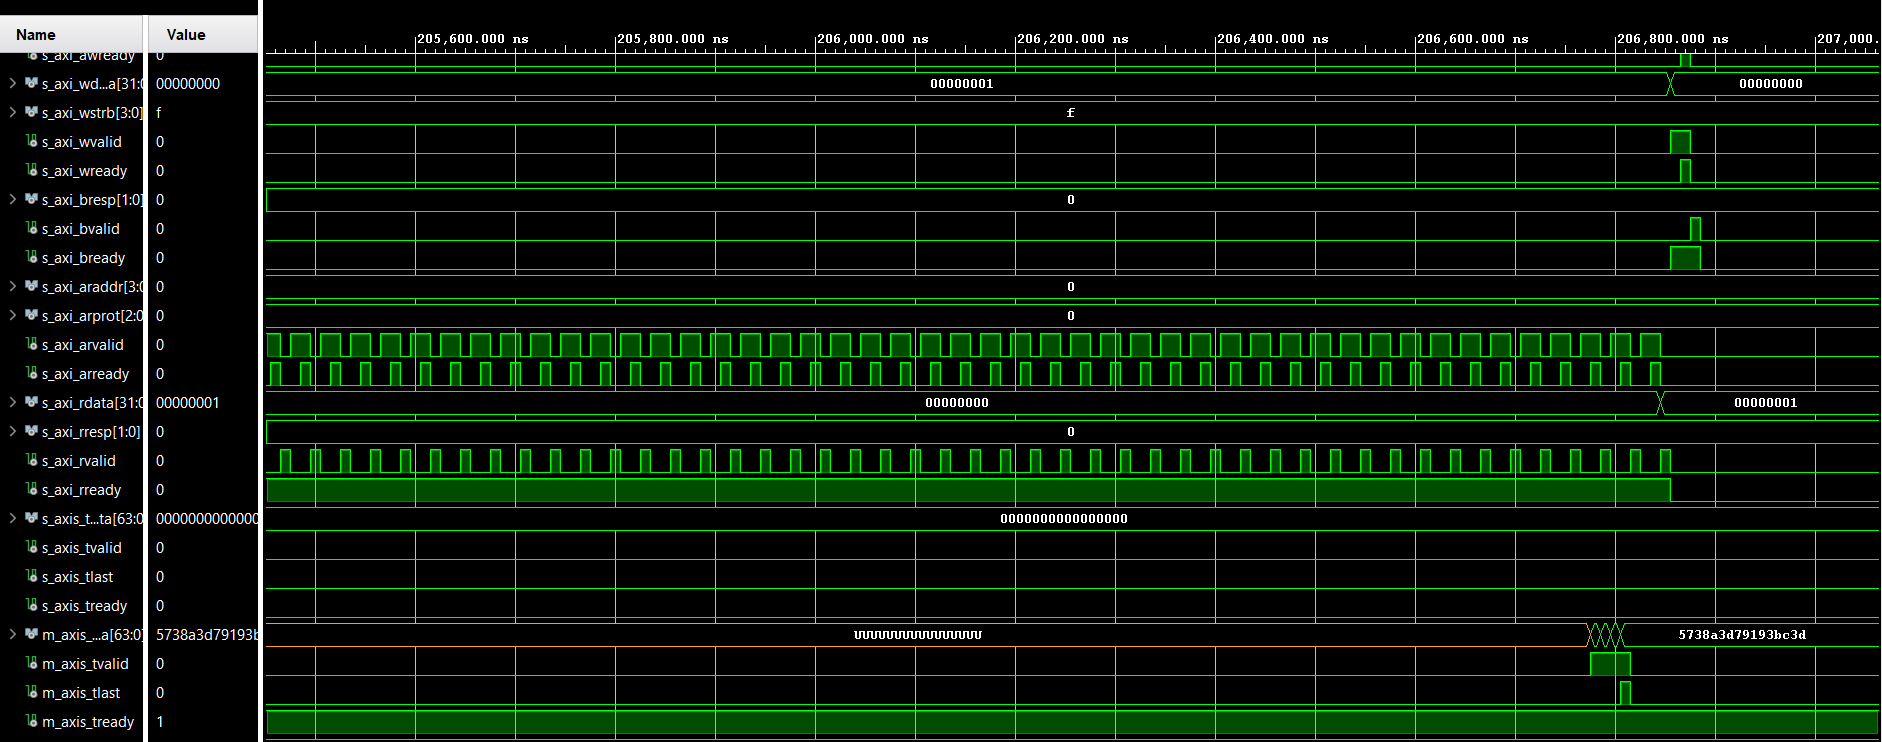
\includegraphics[width=\linewidth]{figures/behavsim_waveform_r2.png}
\caption{Round 2 behavioral simulation waveform showing accelerator activity.}
\label{fig:waveform}
\end{figure}

The captured test logs report 10/10 passing KAT cases for Round 1 and 10/10 passing KAT cases for Round 2 on the Zybo Z7-10. Additional embedded tests for the compiled-in KAT vectors also report pass for both rounds.

\section{Implementation Results}
Vivado 2025.2 reports successful implementation on the \texttt{xc7z010clg400-1} device. Timing is met at a 50 MHz PL clock for both supported rounds. Round 1 has a worst negative slack of 2.496 ns, while Round 2 has a worst negative slack of 2.873 ns. Both timing summaries report zero total negative slack and no failing endpoints. Table~\ref{tab:util} reports the main FPGA resource utilization.

\begin{table}[t]
\centering
\caption{FPGA Resource Utilization on Zybo Z7-10}
\label{tab:util}
\begin{tabular}{lccc}
\toprule
Resource & Round 1 & Round 2 & Available \\
\midrule
Slice LUTs & 15,169 & 15,748 & 17,600 \\
Slice Registers & 10,795 & 10,926 & 35,200 \\
Block RAM Tiles & 23 & 23 & 60 \\
DSPs & 0 & 0 & 80 \\
\bottomrule
\end{tabular}
\end{table}

\begin{figure}[t]
\centering
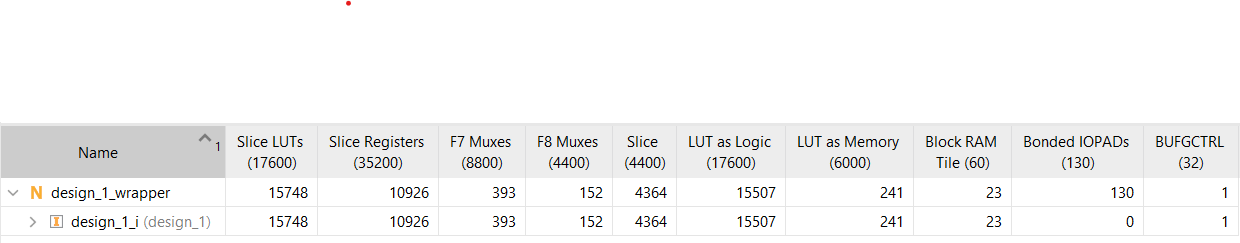
\includegraphics[width=\linewidth]{figures/util_r2.png}
\caption{Round 2 Vivado utilization summary. LUT usage reaches 89.5\% of the target device.}
\label{fig:util}
\end{figure}

The design is LUT-limited on the Zybo Z7-10. Round 1 uses 86.2\% of available LUTs and Round 2 uses 89.5\%. Slice occupancy is effectively near the device limit, with the placed design using more than 98\% of slices for both rounds. BRAM use is moderate at 38.3\%, and no DSP blocks are used. Fig.~\ref{fig:util} shows the Round 2 Vivado utilization summary.

\section{Performance Analysis}
On-board profiling for the Round 1 AXI timer build breaks the total verification time into software, transfer, and hardware phases. Table~\ref{tab:perf} summarizes the measured timing.

\begin{table}[t]
\centering
\caption{Round 1 On-Board Timing Breakdown}
\label{tab:perf}
\begin{tabular}{lc}
\toprule
Operation & Time \\
\midrule
\texttt{mayo\_expand\_pk} & 73.915 ms \\
\texttt{deriveT} & 166.160 us \\
DMA TX (\texttt{SIG+EPK}) & 1116.735 ms \\
Hardware compute & 1.200 us \\
Total & 1190.818 ms \\
\bottomrule
\end{tabular}
\end{table}

The most important result is that the PL computation is very fast relative to the rest of the verification pipeline. The quadratic accumulator completes in about 1.2 microseconds. However, the end-to-end time is dominated by DMA transfer of the expanded public key. For Round 1, the transfer of approximately 99 kB accounts for roughly 93.77\% of the measured total. The AES-based key expansion on the ARM processor is the second-largest contributor at about 73.9 ms.

\section{Source Code}
The code, including VHDL hardware, C software, testbenches, scripts, vectors, KAT files, and reports, is available at \url{https://github.com/kowsyap/mayo-verify-accelerator}.

\section{Conclusion}
The MAYO verification accelerator implements a working FPGA-based hardware/software co-design for both Round 1 and Round 2 Security Level 1 Set 2 instances. The design passes behavioral simulation and on-board Known Answer Tests, meets 50 MHz timing on the Zybo Z7-10, and computes the PL-side verification result in approximately 1.2 microseconds. Resource reports show high LUT utilization, especially for Round 2, but moderate BRAM usage and no DSP consumption. The dominant system bottleneck is not the \(F_q\) arithmetic but the transfer of the expanded public key from PS memory to PL. Future work should therefore focus on reducing EPK movement, caching expanded keys, or selectively moving key expansion into hardware if a larger FPGA target is available.

\begin{thebibliography}{99}

\bibitem{mayo}
W. Beullens, ``MAYO: Practical Post-Quantum Signatures from Oil-and-Vinegar Maps,'' in \emph{Selected Areas in Cryptography -- SAC 2021}, Lecture Notes in Computer Science, vol. 13203, pp. 355--376, Springer, 2022, doi: 10.1007/978-3-030-99277-4\_17.

\bibitem{mayo-r1}
W. Beullens, F. Campos, S. Celi, B. Hess, and M. J. Kannwischer, ``MAYO Specification: Round 1 Version,'' MAYO submission specification, \url{https://pqmayo.org/assets/specs/mayo-round1.pdf}.

\bibitem{mayo-r2}
W. Beullens, F. Campos, S. Celi, B. Hess, and M. J. Kannwischer, ``MAYO Specification: Round 2 Version,'' MAYO submission specification, Feb. 2025, \url{https://pqmayo.org/assets/specs/mayo-round2.pdf}.

\bibitem{nistpqc}
National Institute of Standards and Technology, ``Post-Quantum Cryptography Standardization,'' NIST Computer Security Resource Center.

\bibitem{xilinxzynq}
AMD Xilinx, ``Zynq-7000 SoC Technical Reference Manual,'' product documentation.

\end{thebibliography}

\end{document}
